% !TEX TS-program = pdflatex
% !TEX encoding = UTF-8 Unicode

\documentclass[sigconf]{acmart}
\captionsetup{font=footnotesize}
\usepackage{graphicx}

\settopmatter{printacmref=false} % Removes citation information below abstract
\renewcommand\footnotetextcopyrightpermission[1]{} % removes footnote with conference information in first column
%%\pagestyle{plain} % removes running headers
\thispagestyle{empty}
%%
%% \BibTeX command to typeset BibTeX logo in the docs
\AtBeginDocument{%
    \providecommand\BibTeX{{%
        \normalfont B\kern-0.5em{\scshape i\kern-0.25em b}\kern-0.8em\TeX}}}

\setcopyright{none}
\copyrightyear{}
\acmYear{}
\acmDOI{}

\acmConference[Computer Science]{}{University of Salerno}{UNISA}
\acmBooktitle{Real time Alexa packets profiling analysis}
\acmPrice{}
\acmISBN{}

\begin{document}

    \title{Real time Alexa packets profiling analysis}


    \author{Giuseppe Polese}
    \orcid{0000-0002-8496-2658}
    \email{gpolese@unisa.it}
    \affiliation{
        \institution{Universit\'a degli studi di Salerno}
        \streetaddress{}
        \city{Salerno}
        \state{}
        \country{Italy}
        \postcode{}
    }

    \author{Bernardo Breve}
    \orcid{0000-0002-3898-7512}
    \email{bbreve@unisa.it}
    \author{Stefano Cirillo}
    \orcid{0000-0003-0201-2753}
    \email{scirillo@unisa.it}
    \affiliation{%
        \institution{Universit\'a degli studi di Salerno}
        \streetaddress{}
        \city{Salerno}
        \state{}
        \country{Italy}
        \postcode{}
    }

    \author{Biagio Boi}
    \email{b.boi@studenti.unisa.it}
    \affiliation{
        \institution{Universit\'a degli studi di Salerno}
        \streetaddress{}
        \city{Salerno}
        \state{}
        \country{Italy}
        \postcode{}
    }

    \begin{abstract}
        Nowadays, the introduction of home virtual assistents like Alexa Echo or Google Home became a practice, just considering that over 27\% of families owns one.

        It's obvious that those devices simplified the life by creating a smart house with few money; but what's the impact these devices have on people privacy?
        There are a lot of cases in the United States in which the judge asked to Amazon to provide the recording done by the Echo in order to find helpful
        evidences for the case; so, the question is: "It's possible to prevent the sending of sensible informations to the servers when the weak word is not pronunced?"

        In this project we will profile each packet exchanged between the Alexa Echo and the Server in order to classify the nature of the packets and consequentially we will use a machine learning model to discover when the Echo is sending an inappropriate packet.
    \end{abstract}

    \keywords{data analytics, alexa, packets profiling}


    \begin{teaserfigure}
        \rule{\linewidth}{1mm}
%%  \includegraphics[width=\textwidth]{sampleteaser}
%%  \caption{Insert text here}
%%  \Description{insert description here}
%%  \label{fig:teaser}
    \end{teaserfigure}

%%
%% This command processes the author and affiliation and title
%% information and builds the first part of the formatted document.
    \maketitle


    \section{Introduction}
    The evolution of smart devices over last years has increased exponentially and the introduction of these devices within the house is progressively growing.
    The major problem related to these devices is that usually the privacy is not considered, although there are a lot of regulations (just see the GDPR) that describe how the user data have to be stored and who can access to these data.
    Starting from these two points I decided to understand what happens within the context of smart assistance device such as Alexa Echo.
    Reading on the Amazon Alexa website it's clear how and when they send data to the Amazon Cloud, but in opposition we have some cases in which the recording done by the Echo have been used during the processes in order to extract some evidence.
    In order to clarify this aspect and the role of the smart assistance devices I decided to analyze the outgoing traffic from the device and classify it by considering the environmental conditions.
    The first phase of this analysis consist in understand which kind of packets are sent from the device in order to create a complete dataset of packets sent by the device; during the second phase I try to understand if exist a pattern that identify the packets that souldn't be sent to the Cloud by creating a machine learning model able to identify them.


    \section{State of Art}
    During the last years different research have been done, related to different aspects of the security and privacy within the IoT context.
    F. Z. Berrehili and A. Belmekki \cite{berrehili} have done a study on the Privacy Preservation in the IoT context that shows all the risks directly related to the architecture; in particular, it underlines the need to always guarantee the anonymization of sensibile data by hidding the correlation between the data itself and the person who produced these data (that is also one of the principle of GDPR).
    Despite these studies, there is an huge percentage of devices that do not consider as serious all the aspects related to the privacy, in particular J. Liu and W. Sun \cite{liu} show different attacks againit werables devices at different levels of the ISO/OSI stack and considering different aspects of privacy and security like data integrity, authentication, authroization, etc. The study shows a lot of attacks aim at sniff the packets during the communication in order to collect sensible informations; this seems to be caused from the problem related to the poor encryption mechanisms implemented into the smart devices.


    \section{Alexa architecture \& security}
    The Alexa architecture isn't really easy to explain, we will resume just the keypoint in order to better understand the main functionalities for our purpose.
    \begin{enumerate}
        \item Alexa is always in listening waiting for the wake word to be pronunced to start the recording of the voice;
        \item From the weak word, till the end of commands, Alexa will record the speech and partially sends it to Alexa Voice Service, that can be considered as the brain of Alexa;
        \item Alexa Voice Service will process the audio using Natural Language Processing and Natural Language Understanding in order to retrieve a response for the given request.
        \begin{enumerate}
            \item Natural Language Processing (NLP) improve the Word Segmentation that separate a chunk of continuous text into separate words.
            \item Natural Language Understanding (NLU) is a subtopic of NLP and uses the AI to map text to the meaning\cite{NLU} in order to understand the speech and the request.
        \end{enumerate}
        \item Depending on the sent command, the Voice Service will take an action (turn on the light) or send the information back to the device and Alexa may speech.
    \end{enumerate}
    All the communications between the Echo and the Server are secured by using an SSL/TLS encryption schema.
    In particular, the Echo looks for an available Amazon Server each 3 minutes and then establish a connection (by following the SSL Handshake).
    Once the communication has been initialized it starts to send different packets of different size always encrypted; clearly, these pakcets may contains both authorized and unauthorized data.
    It's important to underline that all the recordings are available on the Amazon platform and can be reproduced and deleted whenever the user wants only by accessing to the platform and this guarantee more transparency to the user that can directly handle all the recordings.
    The point is that here we found only the recordings done by the Echo in an authorized way (when the wake word it's been pronounced), but this doesn't imply that some other recordings can exist and be stored in hidden way.


    \section{Packets analysis}
    In order to create a good dataset we will classify the packets sent by the Echo.
    In particular is possible to classify the type of packet by looking at flags, packet size and protocol used.
    There are different types of packet that will later be included in the dataset as classes:
    \begin{enumerate}
        \item \textbf{handshake}: At the beginning of each new SSL/TLS communication between the Echo and the Server there are different packets exchanged in order to establish a secure communication.
        These packets can be easily identified by the protocol used for the communication (TLS) and by checking the flags related to the content of the message, in particular, the possible flags are:
        \begin{enumerate}
            \item Change Cipher (20).
            \item Server Hello - Show Certificate - Encrypted Message (21).
            \item Alert (22).
        \end{enumerate}
        \item \textbf{syn}: Packets with fixed length are sent from the device in a fixed interval, seems that them are used to synchronize the Echo to the Server.
        \item \textbf{ack}: These are the classical packets used to confirm that the received packets are valid and successfully received.
        \item \textbf{retransmit}: These packets are used to retransmit the data that didn't received an ack, usually this happens when the Echo try to communicate with other Amazon devices (Fire Stick for ex.) but doesn't receive response.
        \item \textbf{app\_data}: These packets are relative to the normal communication of the Echo and can be easily recognized since the communication happens over TLS/SSL protocol and by checking the flag of the considered packet that is equal to 23.
        In particular, we will include in this class all the communication packets that include also recording of voice occurred during the conversation between the Echo and the final costumer.
        \item \textbf{not\_relevant}: We will include in this category all packets that don't match any of the other categories, and are not relevant for our study.
    \end{enumerate}
    It's import to underline that the packets classified as app\_data may include both authorized and not authorized packets.
    The unauthorized packets include all those packets sent in a context in which no application date should be sent to the Server by considering the environmental variables (no wake word pronounced) and hardware aspects (microphone muted by pressing the relative button); for this reason is important to introduce some classes related to these aspects.
    The aim is to distinguish three kind of packets:
    \begin{itemize}
        \item \textbf{not\_justified}: packets sent to the Server in a context in which the Echo is unable to send these data by considering the hardware aspects.
        \item \textbf{justified}: packets sent to the Server without any interaction between the Echo and the Customer, but the Echo is able to listen.
        \item \textbf{expected}: packets sent to the Server since an interaction between the Echo and the Customer happened.
    \end{itemize}
    Clearly, the only allowed packets are those classified as "Expected".
    \subsection[Consideration on packet]{Consideration on packet analysis}
    It's important to do some consideration over the analysis / collection phase just described, in fact there are a lot of behavioural pattern that the Echo follow to perfrom some actions:
    \begin{itemize}
        \item As introduced in the previous section there are some kind of packets that always follow the same schema in a given interval.
        These packets may be sent to guarantee the synchronization with the Amazon Alexa application and with the Amazon servers.
        There are two possible synchronization packets:
        \begin{enumerate}
            \item A packet of 100 byte is sent each 30 seconds (30002 milliseconds)
            \item A packet of 99 byte is sent each 90 seconds (90820 milliseconds)
        \end{enumerate}
        The communication always happens using SSL/TLS, so it's impossible to decrypt the content of these message and confirm that is securely a synchronization packet.
        \item Music stream pattern is dependent on music service used; a stream with Amazon Music always uses a secure connection by using TLS.
        \begin{figure}[h!]
            \centering
            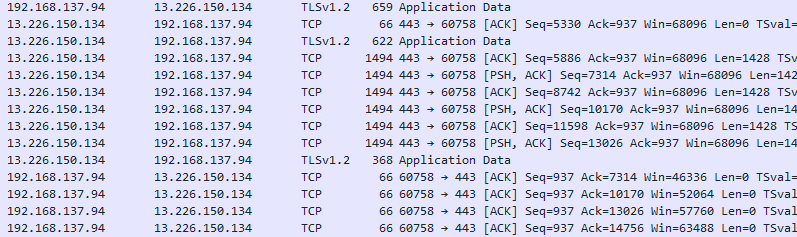
\includegraphics[width=0.8\columnwidth]{img/capture_amazon_music.png}
            \caption{Captured packets during Amazon Music streaming (Wireshark)}
            \label{fig:capture_amazon_music}
        \end{figure}

        Instead, a stream with Spotify makes an HTTP request to Spotify Server that can be captured and replicated
        \begin{figure}[h!]
            \centering
            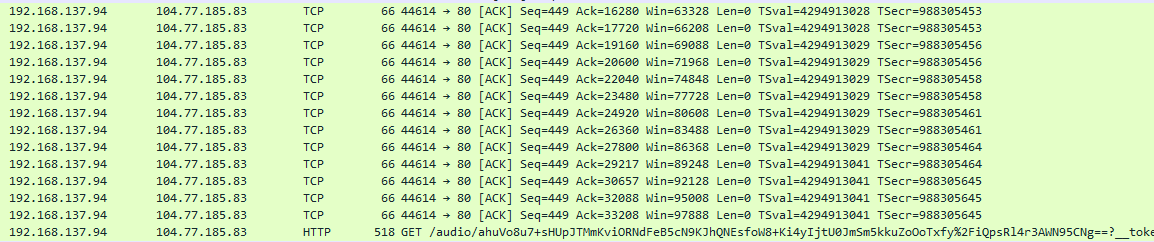
\includegraphics[width=0.8\columnwidth]{img/capture_spotify.png}
            \caption{Captured packets during Spotify streaming (Wireshark)}
            \label{fig:capture_spotify}
        \end{figure}
        \item Echo changes server every 2 minutes, for this reason there are a lot of handshake.
    \end{itemize}


    \section{Dataset}
    In order to create a valid and well-distributed dataset we analyzed the behavior of the Echo in different context, in particular by considering different cases:
    \begin{enumerate}
        \item \textbf{Microphone mute}: when the hardware button is pressed and the device should be unable to send application data to the server.
        \begin{figure}[h!]
            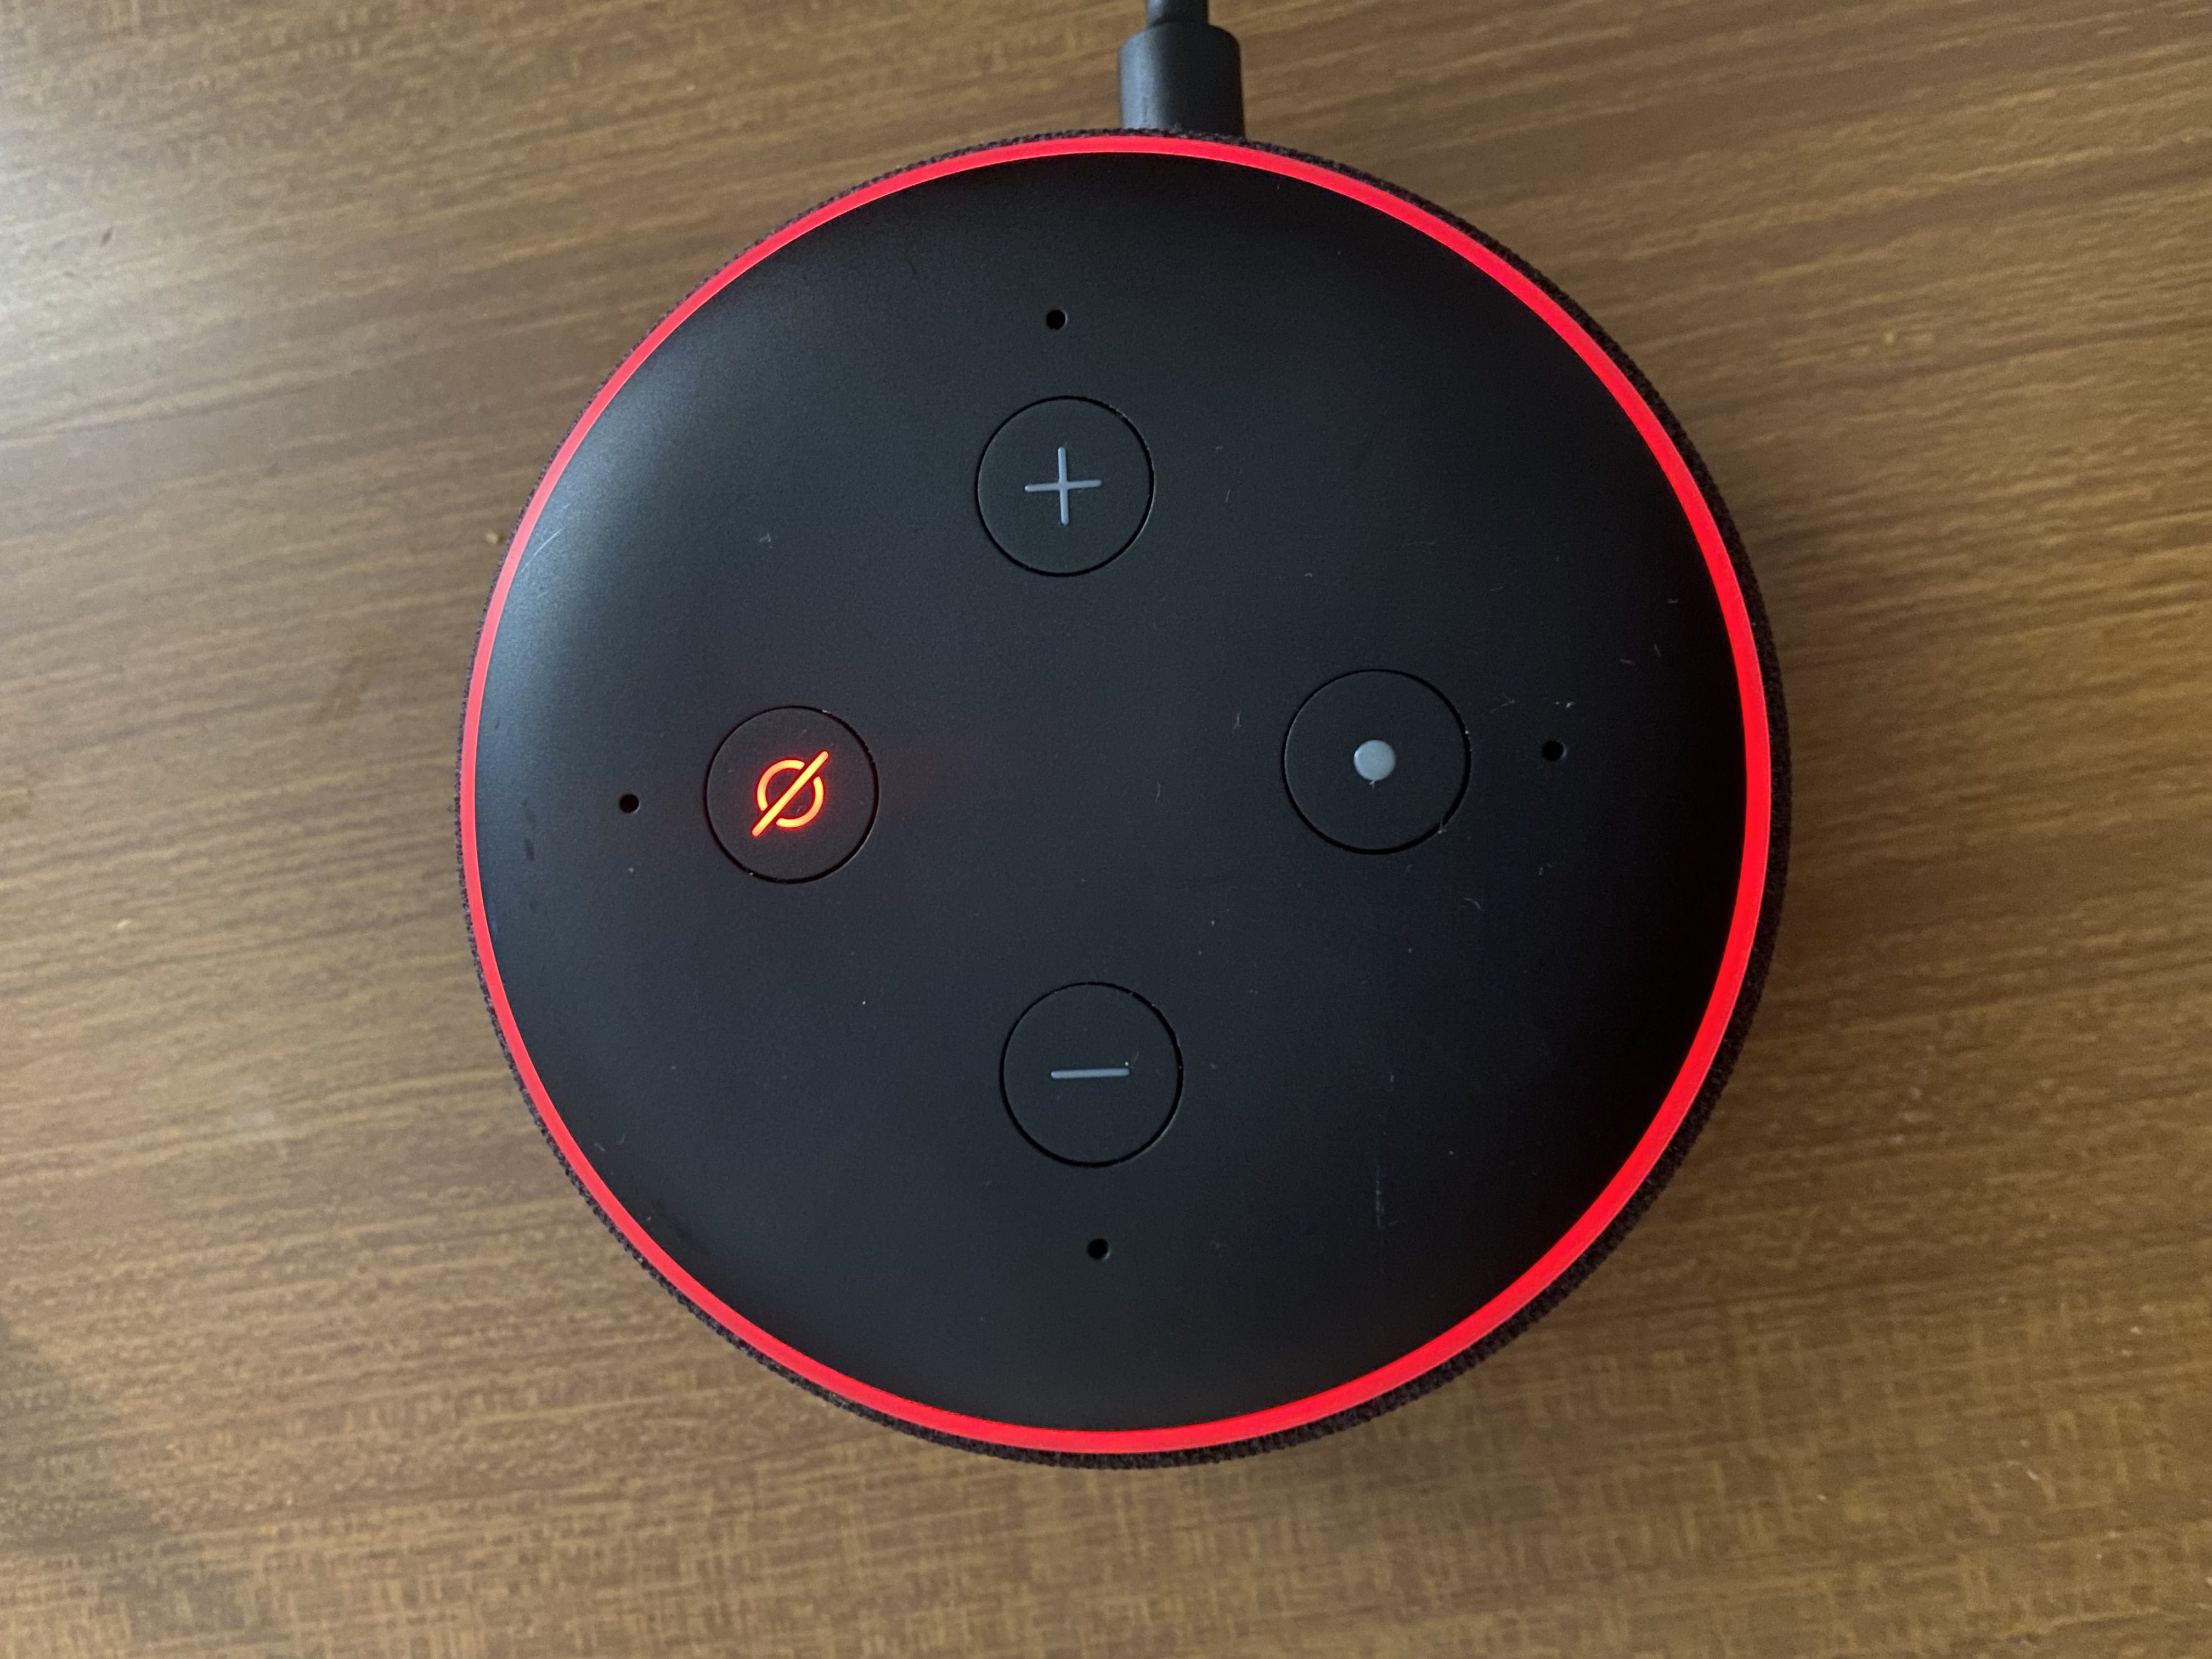
\includegraphics[width=0.8\linewidth]{img/alexa_red.jpg}
            \caption{Echo when the disable microphone button has been pressed.}
            \label{fig:Alexa_red_led}
        \end{figure}
        \item \textbf{No wake word pronounced}: when the device is able to listen the voice but shouldn't send to the Server any packets of application data.
        \item \textbf{Normal stream of data}: when a communication happens.
        It may include different questions or requests, for example:
        \begin{enumerate}
            \item How is the weather today?
            \item When does Liverpool play?
            \item Add milk to the shopping list.
            \item How much is 20 + 20?
        \end{enumerate}
        All these questions or requests expect a response from the Server, so a huge amount of ack will be sent from the device.
        \item \textbf{Streaming}: when the user request for a song and the Echo start to stream it; also in this case a lot of ack packets are sent from the device as response to the fragment of the item to stream (a song for example).
    \end{enumerate}
	\subsection{Considered features}
    As introduced in the previous section it's important to collect features related to both hardware and software aspects; let's see in detail which are the considered features with the related meaning:
    \begin{enumerate}
        \item \textbf{date}: the date in which the packet has been collected, in the format YYYY-MM-DD hh:mm:ss:ms;
        \item \textbf{length}: the length of the packet, it includes just the payload (in case of ack packest it's equal to zero);
        \item \textbf{dstip}: the destination ip, collected to analyze the owner of the server to which the packet is directed;
        \item \textbf{dstport}: the destination port;
        \item \textbf{highest\_layer}: the protocol used, in order to parse the protocol into an integer we will use the following mapping:
        \begin{itemize}
            \item 0 - SSL
            \item 1 - TCP
            \item 2 - DATA
            \item 3 - HTTP
        \end{itemize}
        Notice that all the packets that use other protocol are discarded since them have no meaning for our purpose;
        \item \textbf{delta}: the time occured from the previous packet of the same stream;
        \item \textbf{ack\_flag}: the acknowledge flag; it is equal to 1 if the packet contains an ack;
        \item \textbf{microphone}: the status of the microphone, it is equal to 1 if the microphone is active, 0 otherwise;
        \item \textbf{content\_type}: the type of content sent, it is valorized only if the packet is sent over SSL;
        \item \textbf{synchronized}: status of sychronization of the device, it is equal to 1 if the Echo has been previously associated to an account, 0 otherwise.
    \end{enumerate}
    Since we want to map every kind of packet in a class, 8 classes have been declared: handshake, syn, ack, retransmit, not\_relevant, justified, not\_justified and expected. 
	\subsection{Dataset composition}
	Once we have explained which are the considered features, let's have an overview on the dataset composition by analyzing the features and classes distriburions.


    \section{Machine learning}
    TODO


    \section{Conclusions}
    TODO

    \bibliographystyle{plain}
    \bibliography{biblio_ref}

\end{document}
\endinput
%%
%% End of file `sample-sigconf.tex'.
